%# -*- coding: utf-8-unix -*-
%%==================================================
%% chapter01.tex for SJTU Master Thesis
%%==================================================

%\bibliographystyle{sjtu2}%[此处用于每章都生产参考文献]
\chapter{系统实现}
\label{chap:sys_impl}
我们利用Docker \emph{swarm}作为容器云的具体实现,基于Docker 17.04.0-ce版本实现了本文提出的模型。图\ref{fig:swarmkit-modify}显示了以Docker \emph{swarm}框架实现的容器云中服务的创建过程:
\begin{figure}[htbp]
\centering
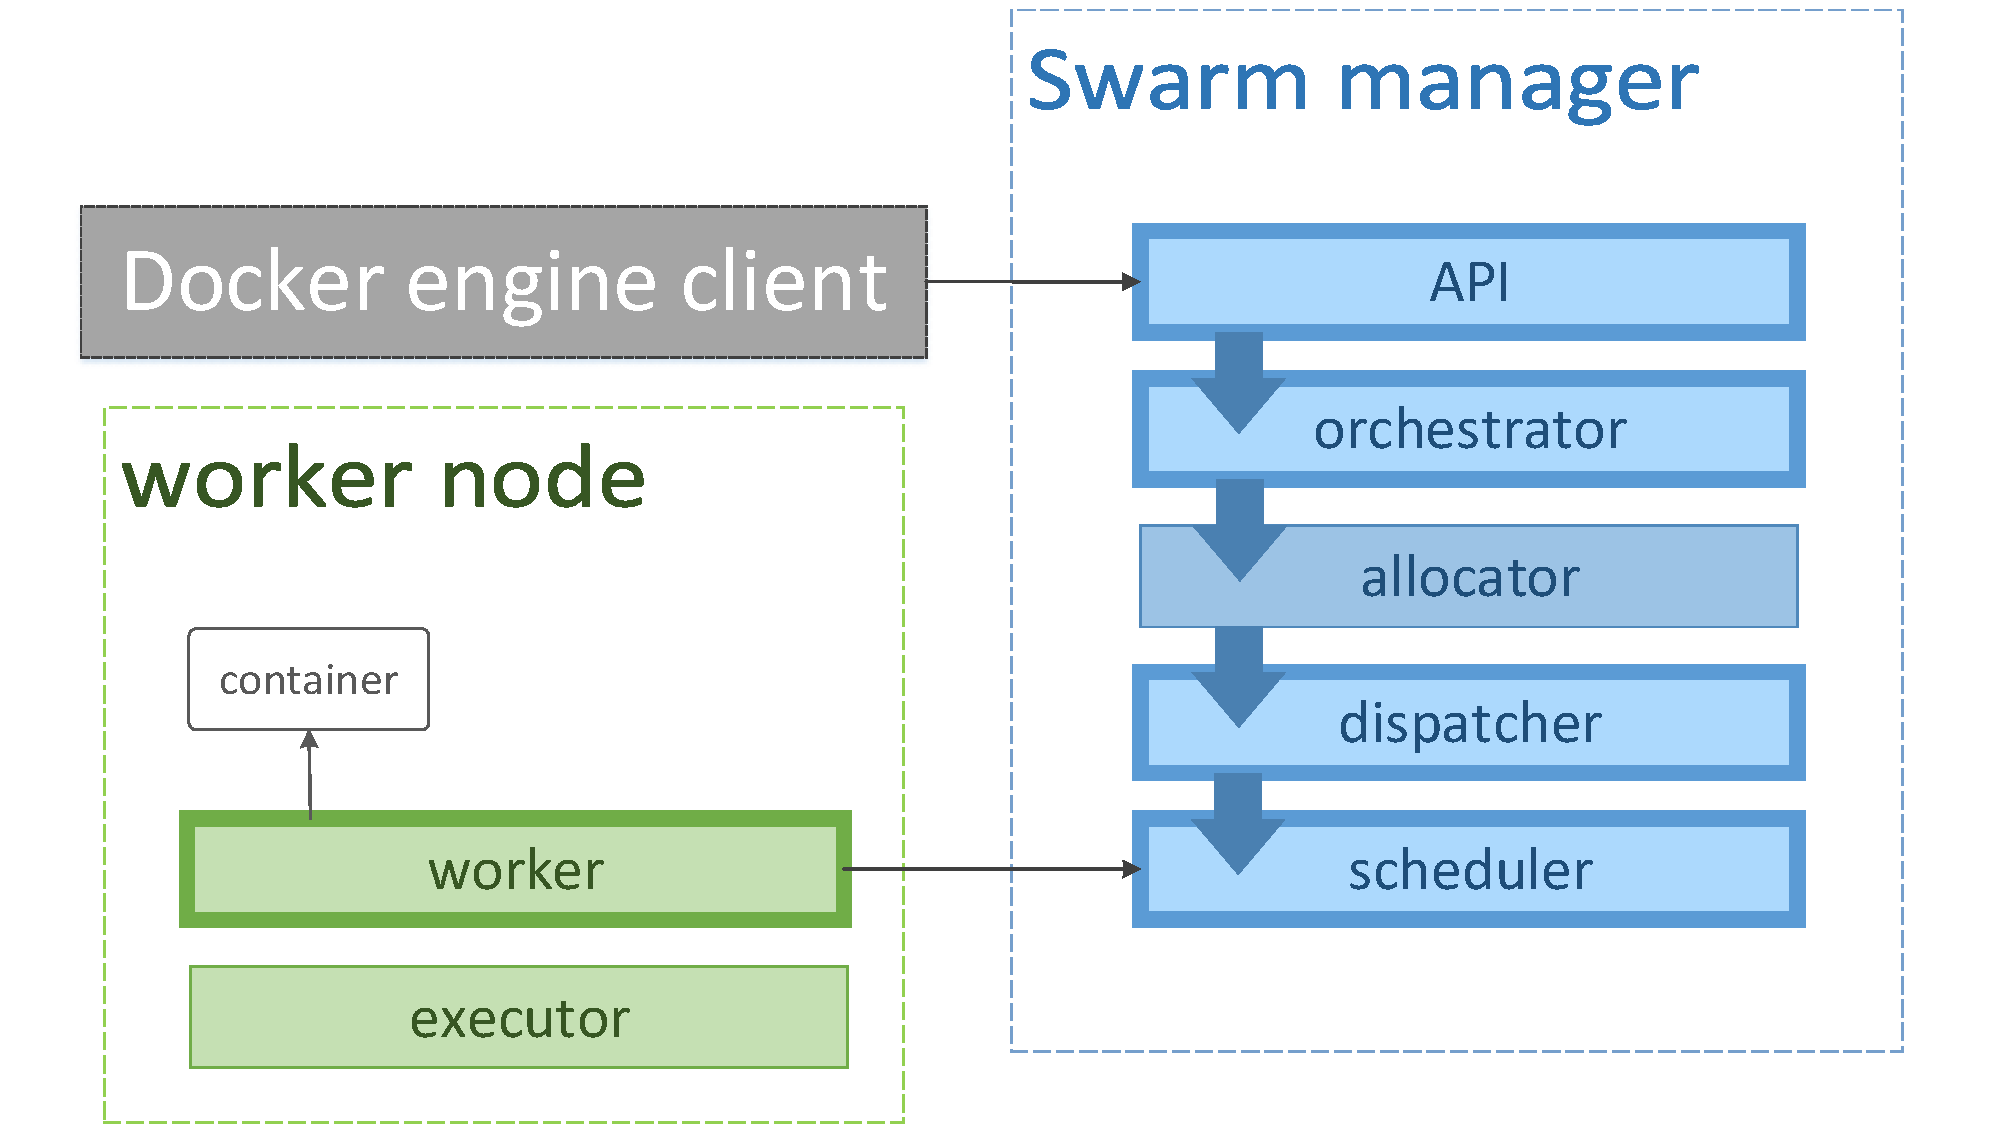
\includegraphics[width=0.9\textwidth]{./figure/modification}
\bicaption[fig:swarmkit-modify]{服务创建过程}{\textbf{服务在基于Docker \emph{swarm}实现的容器云中的创建过程}}{Fig}{\textbf{Service Creation Process}: creating service with Docker \emph{swarm}}
\end{figure} 

在管理者节点上,API模块负责解析用户从客户端发起的请求,orchestrator模块保证相应服务有满足要求的任务实例在集群中运行,allocator模块负责分配网络和硬盘等资源,dispatcher模块负责保持工作者节点和管理者节点之间的通信,scheduler模块则根据调度规则分配任务到各个工作者节点。
在工作者节点上,worker模块负责管理和运行实际运行相关任务实例的容器,agent模块负责跟踪任务实例的运行状态并将状态同步给管理者节点。

\section{各模块详细实现}

\subsection{资源使用状态监测模块}
\begin{figure}[!htp]
    \centering
    \resizebox{6cm}{!}{\input{figure/example/flow_chart.tex}}
    \bicaption[fig:flow_chart]{绘制流程图效果}{流程图}{Fig}{Flow chart}
\end{figure}

\subsection{资源使用状态预测模块}

\subsection{资源供给方案生成模块}

A new constraint is introduced to indicate the replica requirements of a service that is supposed to meet its availability requirements. 

\subsection{资源供给优化模块}

\subsection{资源管理模块}

The dispatcher periodically collects certain information from worker nodes in the swarm, such as tasks status and image layer digests on the nodes, and later shares the information with the scheduler.

When a service is created or updated, the orchestrator will put tasks into a task pool and query Docker registry asynchronously for the digests of layers in the corresponding image. Digests of layers can be retrieved by querying correlative image's manifest information from Docker registry.

\subsection{负载优化模块}
The ABP scheduler runs on the manager node having the leadership role of the swarm. The scheduler tries to schedule all tasks in the task pool at regular intervals, following scheduling rules defined in the scheduling algorithm to make schedule decisions. The scheduling algorithm will be discussed in detail in the following section.

In our design, we follow the original process in Docker swarm for the creation and spread of services and make following modifications to implement the ABP scheduler: 

\begin{enumerate}
\item A new constraint is introduced to indicate the replica requirements of a service that is supposed to meet its availability requirements. 
\item The dispatcher periodically collects certain information from worker nodes in the swarm, such as tasks status and image layer digests on the nodes, and later shares the information with the scheduler.
\item When a service is created or updated, the orchestrator will put tasks into a task pool and query Docker registry asynchronously for the digests of layers in the corresponding image. Digests of layers can be retrieved by querying correlative image's manifest information from Docker registry. 
\item The ABP scheduler runs on the manager node having the leadership role of the swarm. The scheduler tries to schedule all tasks in the task pool at regular intervals, following scheduling rules defined in the scheduling algorithm to make schedule decisions. The scheduling algorithm will be discussed in detail in the following section.
\end{enumerate}



\section{本章小结}